\documentclass[twoside]{article}

\usepackage{mystyle}
\usepackage{tikz}
\usetikzlibrary{positioning}
\setlength{\belowcaptionskip}{-10pt} % https://tex.stackexchange.com/questions/23313/how-can-i-reduce-padding-after-figure

\title{Machine Learning for Data Science - Competition 2}
\author{Antoine Klopocki, Jaydev Kshirsagar, Travis Westura, Vishisht Tiwari\\Kaggle Team Name: Antravishjay}
\date{\vspace{-5ex}} % vspace hack to remove date without looking into titling package

\begin{document}

\maketitle
\thispagestyle{empty}

\section{Introduction}\label{sec:introduction}

In this competition we are given a robot that is moving around in~$\R^2$.
The robot makes $\num{10000}$~runs, and for $\num{1000}$~timesteps we observe the angle~$\theta'$ that the robot's position makes with the $x$-axis.
But we are not given the robot's precise ${(x, y)}$~location, and the angle itself does not determine directly the robot's position.
The true position could be anywhere along the line determined by $\theta'$.
Our task is to determine the robot's ${(x, y)}$-position on the $\num{1001}$st~timestep as accurately as possible, with accuracy determined by Root Mean Square Error.
Our methods achieve an accuracy score of~$\bm{0.26233}$.

In this report we first give an overview of our model, how it fits the problem, and how we design the algorithms that we use.
We explain the inputs our algorithms take and how we adjusted the input parameters, how we use both the labeled and unlabeled points in the model, and how our failures guided the further development of our algorithms and their implementations.
Throughout the report we include images and explanations of the visualizations we use as we develop our final model.

\section{Visualization and Problem Description}\label{sec:vis-and-prob-desc}

\subsection{Conventions}\label{sec:conventions}

The competition specification describes the robot moving in the first quadrant, and the angles given in the observations file contain the angle made between the robot's location~${(x_{r, t}, y_{r, t})}$ and the horizontal axis passing through a point at which an observer measures the angle the robot's position makes with that axis.
We differentiate between two coordinate systems in our notation using the following conventions:
\begin{wrapfigure}{o}{0.46\textwidth}
  \centering
  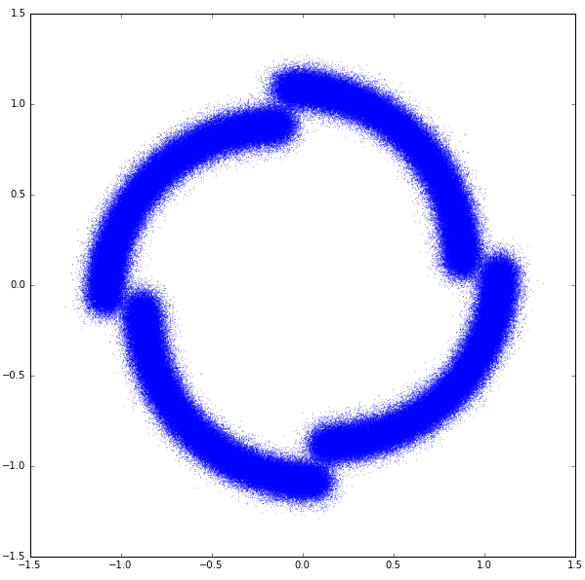
\includegraphics[width=0.45\textwidth]{images/AK1}
  \caption{Locations of the robot given as labels.}\label{fig:label-locations}
\end{wrapfigure}
\begin{itemize}[topsep=2pt]
\item ${(O, x, y)}$ is the system of coordinates of the robot, equal to the coordinates given by the labels.
\item ${(O', x', y')}$ is the system of coordinates of the angle observer, in which the robot makes an angle~$\theta$ to the axis~$X'$.
\end{itemize}
What is the relation between ${(O, x, y)}$ and ${(O', x', y')}$?
The first visualization step is to plot the labels, as in \cref{fig:label-locations}.
The robot appears to follow an almost circular orbit, with a few kinks, of radius~$1$ centered at~$(0, 0)$.

Consider a labeled point~${(x_{r, t}', y_{r, t}')}$.
The angle~$\theta$ that this point forms with the $x$-axis is given by
\begin{equation*}
  \tan\theta = \frac{b + y_{r, t}'}{a + x_{r, t}'}.
\end{equation*}
We know the value of $\theta$ from the observations file.
Since there are two unknowns $a$~and~$b$, we pick two labeled points and solve the system of equations
\begin{equation*}
  \tan\theta_1 = \frac{b + y_{r_1, t_1}'}{a + x_{r_1, t_1}'}, \quad \tan\theta_2 = \frac{b + y_{r_2, t_2}'}{a + x_{r_2, t_2}'}.
\end{equation*}
\begin{figure}[h]
  \centering
  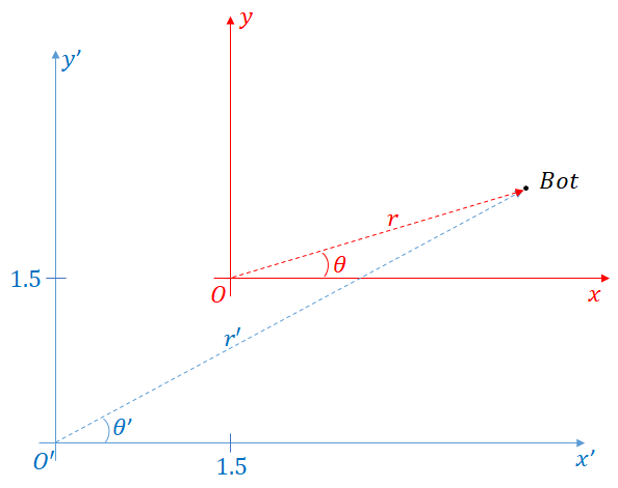
\includegraphics[width=0.40\textwidth]{images/AK2}
  \caption{Conventions of our two coordinate systems.}\label{fig:conventions}
\end{figure}
We use the points from run~$1$ time steps $205$~and~$216$.
Solving the system of equations yields the position of the angle observer as~$(-1.5, -1.5)$ in the ${(O, x, y)}$ coordinate system.
As our intuition about the robot's movement is that it follows a roughly circular orbit centered at ${(x, y) = (0, 0)}$, we introduce the polar coordinates $\theta$ and $r$ in the system ${(O, x, y)}$.
Using this position, we consider the observation angles as being measured at~$(0, 0)$.
We summarize the conventions in \cref{fig:conventions}.

\subsection{Visualization of Consecutive Labels}\label{sec:visu-cons-labels}

To gain more intuition about the behavior of the robot, we further focused on the consecutive labels, that is, the labels that occur in the same run at two consecutive time steps.
We found $\num{68666}$~consecutive labels out of $\num{600000}$~labels, which enable us to form a representation of their behavior.
For each such consecutive labeled point~${(x, y)}$, we compute the polar representation~${(r, \theta)}$ and plot histograms of their distributions.
Further, we calculate also ${\dif r}$ and~${\dif \theta}$, which are the differences between the respective values of the consecutive points.
These histograms are given in \cref{fig:histograms}.
\begin{figure}[h]
  \centering
  \begin{subfigure}[h]{0.4\textwidth}
    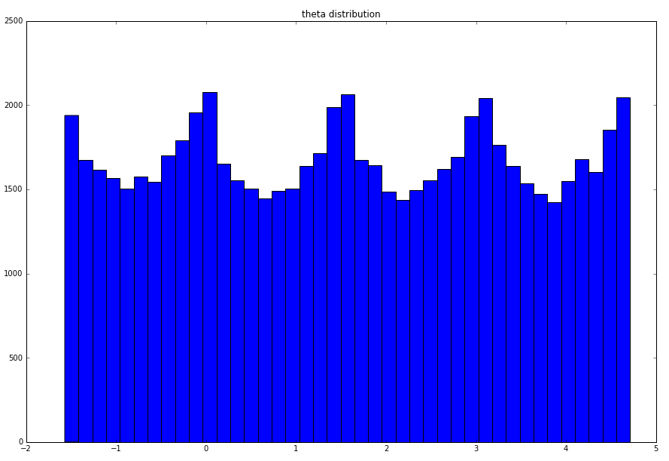
\includegraphics[width=\textwidth]{images/AK3}
    \caption{$r$}\label{fig:hist-r}
  \end{subfigure}
  \begin{subfigure}[h]{0.4\textwidth}
    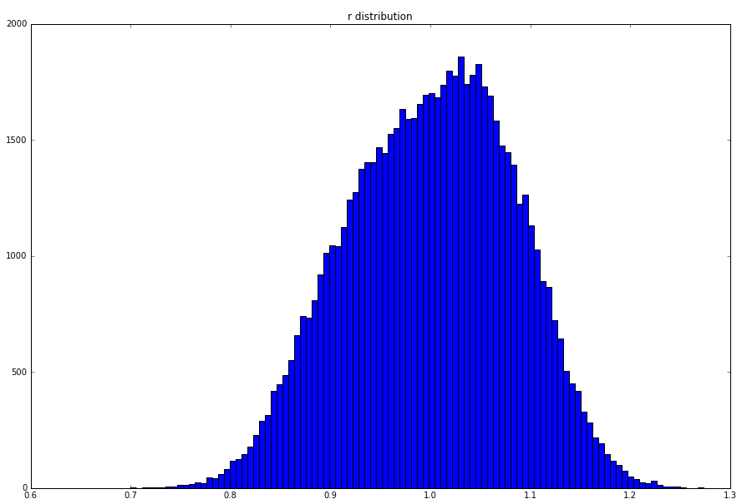
\includegraphics[width=\textwidth]{images/AK4}
    \caption{$\theta$}\label{fig:hist-theta}
  \end{subfigure}\\[2ex]
  \begin{subfigure}[h]{0.4\textwidth}
    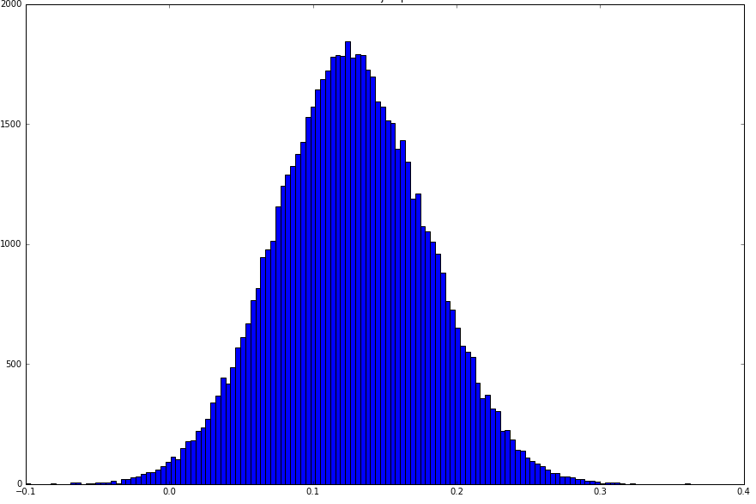
\includegraphics[width=\textwidth]{images/AK5}
    \caption{$\dif r$}\label{fig:hist-dr}
  \end{subfigure}
  \begin{subfigure}[h]{0.4\textwidth}
    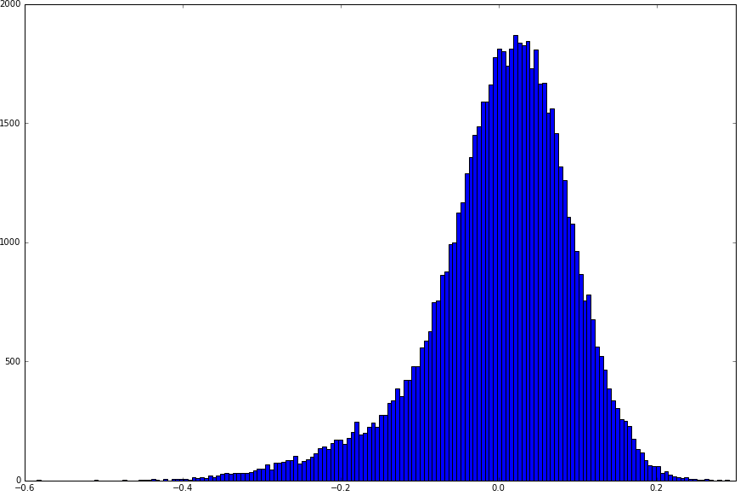
\includegraphics[width=\textwidth]{images/AK6}
    \caption{$\dif \theta$}\label{fig:hist-dtheta}
  \end{subfigure}
  \caption[histograms]{Histograms of $r$,~$\theta$,~${\dif r}$, and~${\dif \theta}$.}\label{fig:histograms}
\end{figure}
From these observations, we infer a great deal of useful information about the problem:
\begin{itemize}
\item The robot is turning counterclockwise (increasing values of $\theta$).
  From \cref{fig:hist-dtheta}, however, there are some rare cases where ${\dif \theta}$ is negative, corresponding to steps where the robot turned clockwise.
\item ${\dif \theta}$ seems to follow a normal distribution of mean~$0.125$ and variance~$0.2$.
  We make an assumption that ${\dif \theta}$ is independent from both $r$ and from $\theta$ (symmetry of revolution), that is, the $\theta_{t+1}$ of step ${t+1}$ is chosen form a normal distribution of mean~${\theta_t + 0.125}$ and variance~$0.2$.
\item ${\dif r}$ seems to be a bit more complicated.
  It most cases it seems to follow a normal distribution of mean~$0.0231$, and when $\theta$ has a certain value ($\theta \approx 0 \bmod \frac{\pi}{2}$), ${\dif r}$ is negative (there is a kink in the path and a jump to a lower $r$).
\end{itemize}
Having normal distributions is consistent with the fact that we know the bot is moving continuously in~$\R^2$.
We expand upon these observations in \cref{sec:finding-1001-angles}.

\section{Hidden Markov Models (HMM's)}\label{sec:hidden-markov-models}

We represent this problem as a Hidden Markov Model.
A Hidden Markov Model is a graphical model with two types of variables: latent variables~$S_t$ and observed variables~$X_t$.
The latent variables represent states that are not visible to the observer.
Each observed variable~$X_t$ depends only on the corresponding state variable~$S_t$.
And each state variable~$S_t$ depends only on the previous state variable~$S_{t-1}$.
We depict latent variables as shaded vertices.

\begin{figure}[h]
  \centering
  \tikz[]{
    \node[draw, circle, fill=gray] (S1) {$S_1$};
    \node[draw, circle] (X1) [on grid, below = 1.5cm of S1] {$X_1$};
    \node[draw, circle, fill=gray] (S2) [on grid, right = 1.5cm of S1] {$S_2$};
    \node[draw, circle] (X2) [on grid, below = 1.5cm of S2] {$X_2$};
    \node[] (dots) [right = 0.7cm of S2] {$\cdots$};
    \node[draw, circle, fill=gray] (Sn) [on grid, right = 1.5cm of dots] {$S_T$};
    \node[draw, circle] (Xn) [on grid, below = 1.5cm of Sn] {$X_T$};

    \path[shorten >=0.1cm, shorten <=0.1cm, ->] (S1) edge (X1);
    \path[shorten >=0.1cm, shorten <=0.1cm, ->] (S1) edge (S2);
    \path[shorten >=0.1cm, shorten <=0.1cm, ->] (S2) edge (X2);
    \path[shorten >=0.1cm, shorten <=0.1cm, ->] (S2) edge (dots);
    \path[shorten >=0.1cm, shorten <=0.1cm, ->] (dots) edge (Sn);
    \path[shorten >=0.1cm, shorten <=0.1cm, ->] (Sn) edge (Xn);
  }
  \caption{Hidden Markov Model}\label{fig:hmm}
\end{figure}

While an HMM seemed to be the most appropriate way of modelling the problem, one essential difference that exists between the target problem and the typical HMM use cases is that the hidden as well as the observed random variables are continuous, unlike the discrete nature in case of other HMM applications.
We decided to use discretization to overcome this difficulty.
But this method is subject to the error that is introduced because of the quantization, and consequently larger steps give worse accuracy.
We searched for prior work done for developing HMM variants that deal with continuous random variables.
We found one paper that described HMMs with continuous-time, and another one that described HMMs with the observations as continuous random variables.
The latter seemed better suited for the target problem since the timesteps are discrete and the observations continuous.
The approach models observation probabilities as continuous density functions, generally a Gaussian, the Emission probabilities get expressed in terms of the parameters of the distribution.
These parameters are the mixture coefficient---the mean and the covariance---which are learnt during the E-M process.
Although the approach seemed convincing from the point of view of the accuracy, it was evident that this would involve an increased amount of computation as compared to the discrete HMM version, since there are 3 parameters to be learned instead of the single entry in the Emission table cells.
Further, the number of floating point operations would increase, as we would be dealing with the probability density functions.
Given that we were facing a challenge with the running time and numerical stability of the the discrete version itself, we de-prioritized the actual implementation of the continuous HMM and considered it as an option to look out for increasing accuracy once the discrete model gave satisfactory results.

In our problem the observed values are the angles that the robot's position makes with the $x$-axis.
The robot is moving around in the plane~$\R^2$.
This space is continuous, so our observations are angles in the continuous range~$\big(0, \frac{\pi}{2}\big)$.
We discretize this space in order to use a Hidden Markov Model.
We divide the first quadrant into $K$~sectors, ${\textstyle \big[0, \frac{1}{K}\frac{\pi}{2}\big), \big[\frac{1}{K}\frac{\pi}{2}, \frac{2}{K}\frac{\pi}{2}\big), \ldots, \big[\frac{K - 1}{K}\frac{\pi}{2}, \frac{\pi}{2}\big)}$, where $K$ is a parameter that we choose.
The observation, rather than being a value in $\big(0, \frac{\pi}{2}\big)$, is instead given by an integer~${1, 2, \ldots, K}$ representing the segment of the interval in which the angle lies.
As a further refinement of this technique, we find the minimum and maximum angles that occur in the observations file, $\theta_{\text{min}}$~and~$\theta_{\text{max}}$, and divide the shorter interval~$[\theta_{\text{min}}, \theta_{\text{max}}]$.

\begin{wrapfigure}{o}{0.5\textwidth}
  \begin{center}
    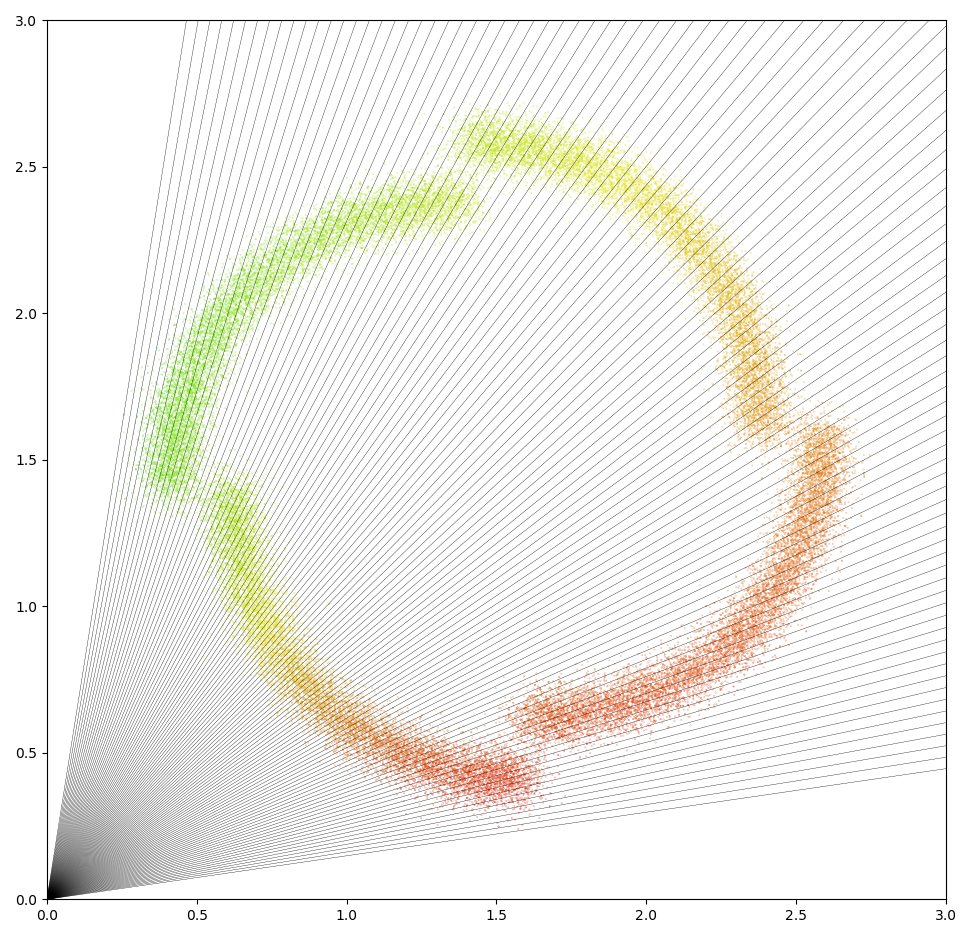
\includegraphics[width=0.48\textwidth]{images/angle-discrete}
    \caption{Labeled points colored based on the segment in which they lie with~${K = 100}$.}
  \end{center}
\end{wrapfigure}

Given an observation and the corresponding state, we need to map the state to the robot's position.
We outline a procedure for doing this in \cref{sec:using-labels-map}.

Given the observations, we need to estimate the transition matrix~$A$ and emission matrix~$B$ of the Hidden Markov Model.
The transition matrix is defined by
\begin{equation*}
  a_{i,j} = \Pr(S_{t} = j \mid S_{t-1} = i),
\end{equation*}
that is, each entry~$a_{i, j}$ gives the probability of being in state~$i$ given that the previous state is state~$j$.
With $N$~states, $A$ is an ${N \times N}$-matrix.
The emission matrix is defined by
\begin{equation*}
  b_{i, k} = \Pr(X_t = k \mid S_t = i),
\end{equation*}
that is, each entry~$b_{i, k}$ gives the probability of the observation~$k$ being emitted given state~$i$.
With $N$~states and $K$~possible observations, $B$ is an ${N \times K}$-matrix.
In~\cref{sec:baum-welch} we describe our process for estimating these matrices using the Baum Welch algorithm.

\section{Algorithms and Implementation}\label{sec:algo-and-impl}

We model this problem as an HMM learning problem, where we need to use and algorithm to learn the transition, emission, and initial probabilities.
Our main tool is the Baum Welch algorithm.

\subsection{Baum Welch}\label{sec:baum-welch}
The Baum Welch algorithm is an Expectation Maximization (EM) algorithm for learning the parameters of Hidden Markov Models.
We use a forward-backwards algorithm to perform inference for the expectation step and then update the HMM parameters in the maximization step.
We thereby find the maximum likelihood estimate of the parameters of the model.
The algorithm takes as parameters a triple~$(A, B, \pi)$, where $A$~and~$B$ are the transition and emission matrices and $\pi$ is the initial state distribution, that is, the probability of the first state being state~$i$ is given by ${\pi_i = \Pr(S_1 = i)}$.

\subsubsection{Our Implementation of Baum-Welch}\label{sec:expl-algor}

To achieve a high accuracy, we develop our own Baum-Welch algorithm.
After using the basic implementation, we tweak the alogrithm to achieve better results.

\paragraph{Description of Algorithm}

Let $N$ be the number of states, $K$ be the number of observations, and $T$ be the number of time steps.

For the forward procedure we calculate ${\alpha_i(t) = \Pr(X_1 = x_1, X_2 = x_2, \ldots, X_t = x_t, S_t = i \mid A, B, \pi)}$, which is the probability of obtaining observations~${y_1, y_2, \ldots, y_t}$ and being in state~$i$ at time~$t$.
We recursively compute
\begin{align*}
  \alpha_i (1) &:= \pi_i b_{i, x_1},\\
  \alpha_i (t + 1) &:= b_{i, x_{t+1}} \sum_{j=1}^N \alpha_j(t) a_{j, i}.
\end{align*}
For the backward procedure we calculate ${\beta_i(t) = \Pr(X_{t+1} = x_{t+1}, \ldots, X_T = x_T \mid S_t = i, A, B, \pi)}$, the probability of the observations ${x_{t+1}, \ldots, x_T}$ occurring given the $t$th~state is state~$i$.
Again we compute recursively to set
\begin{align*}
  \beta_i(T) &:= 1,\\
  \beta_t(t) &:= \sum_{j=1}^N \beta_j(t+1) a_{i, j} b_{j, x_{t+1}}.
\end{align*}

Before performing the updates, we first calculate two temporary variables.
We define $\gamma_i(t)$ to be the probability of being in state~$i$ at time~$t$ given a set of observations~${X = (X_1 = x_2, \ldots, X_T = x_T)}$.
Applying Bayes's theorem we have
\begin{equation*}
  \gamma_i(t) := \Pr(S_t = i \mid X, A, B, \pi) = \frac{\Pr(S_t = i, X \mid A, B, \pi)}{\Pr(X \mid A, B, \pi)} = \frac{\alpha_{i}(t) \beta_i(t)}{\sum_{j = 1}^N \alpha_j(t) \beta_j(t)}.
\end{equation*}
Next we define $\xi_{i, j}(t)$ to be the probability of being in state~$i$ at time~$t$ and state~$j$ at time~$t + 1$ given a sequence of observations~$X$ with parameters $A$,~$B$, and~$\pi$.
\begin{align*}
  \xi_{i, j}(t) &:= \Pr(S_t = i, S_{t+1} = j \mid X, A, B, \pi) = \frac{\Pr(S_t = i, S_{t+1} = j, X \mid A, B, \pi)}{\Pr(X \mid A, B, \pi)},\\
  &= \frac{\alpha_t(t) a_{i, j} \beta_j(t + 1) b_{j, t+1}}{\sum_{i=1}^N \sum_{j=1}^N \alpha_i(t) a_{i, j} \beta_j(t+1) b_{j, t+1}}.
\end{align*}
We use these temporary variables to update the parameters of our Hidden Markov Model.
The vector~$\pi$ is updated so each entry~$\pi_i$ is the probability of being in state~$i$ at the first time~${t = 1}$.
\begin{equation*}
  \pi_i := \gamma_i(1)
\end{equation*}
The values~$a_{i, j}$ are updated to be the expected number of transitions from state $i$~to~$j$ divided the total number of transitions from~$i$ (including from $i$ back to itself).
\begin{equation*}
  a_{i, j} := \frac{\sum_{t=1}^{T-1}\xi_{i, j}(t)}{\sum_{t=1}^{T-1}\gamma_i(t)}
\end{equation*}
And finally the values~$b_{i, k}$ is set to the expected number of times the observation~$k$ is emitted from state~$i$ over the total number of times state~$i$ occurs.
\begin{equation*}
  b_{i,k} := \frac{\sum_{t=1}^T \1_{X_t = k}\gamma_i(t)}{\sum_{t=1}^T \gamma_i(t)}
\end{equation*}

\subsubsection{Implementation on a small dataset}\label{sec:impl-small-data}

We implement this algorithm in Python and first test it with a small data set of $2$~states and $3$~observation types.
We randomize the initial values of our parameters $A$,~$B$, and~$C$ and run for $100$~iterations.
The algorithm proves to be able to predict the states quite accurately.
\Cref{fig:bw-gamma} shows that the $\gamma$~values showing the probability of being in state $1$~or~$2$ at time~$t$ closely follow the observation values.
\begin{figure}[h]
  \centering
  \begin{subfigure}[t]{0.9\textwidth}
    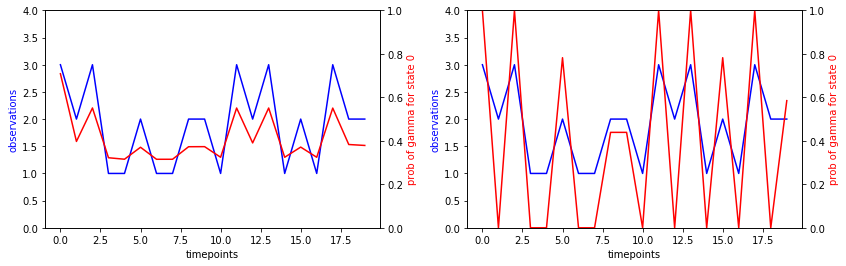
\includegraphics[width=\textwidth]{images/small-dataset-top}
    \caption{Initial observations and value of $\gamma_0$ compared to the values after $100$ iterations of Baum-Welch.}\label{fig:small-dataset-top}
  \end{subfigure}
  \begin{subfigure}[t]{0.9\textwidth}
    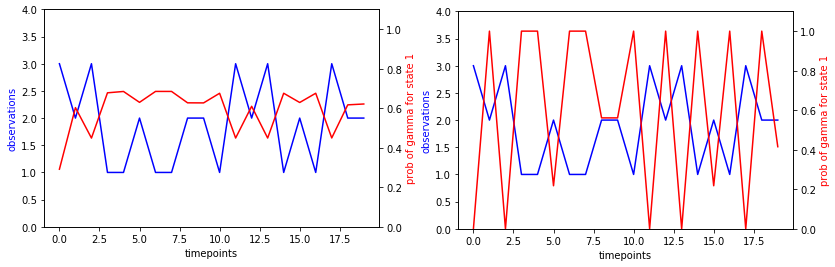
\includegraphics[width=\textwidth]{images/small-dataset-bottom}
    \caption{Initial observations and value of $\gamma_1$ compared to the values after $100$ iterations of Baum-Welch.}\label{fig:small-dataset-bottom}
  \end{subfigure}
  \caption[bw-gamma]{Change in $\gamma$ value during Baum-Welch.}
  \label{fig:bw-gamma}
\end{figure}

\subsubsection{Implementation on the Robot Challenge}\label{sec:impl-robot-challenge}

After testing our implementation with a small parameter size, we attempt to use it to determine the HMM parameters of the robot challenge.
Because the robot moves in a continuous space, we discretize the space so that our algorithm, which accepts discrete inputs, can handle it.
We first tried using large parameters, setting the number of states~${N = \num{3000}}$ and the number of observations~${K = \num{1570}}$.
We round all observation angles to $3$~decimal places to fit our discretization model.
The algorithm runs as follows
\begin{enumerate}
  \item Randomly initialize the transition, emission, and initial probability matrices using $\num{3000}$~states and $\num{1570}$~observations.
  \item Use the Baum Welch algorithm on the first run of the robot with a maximum of $\num{100}$ iterations.
  \item Obtain the new transition, emission, and initial probability matrices as the result.
  \item Repeat for all $\num{10000}$~runs, updating the parameters with each run.
\end{enumerate}

\paragraph{Results}

This experiment fails to produce a suitable result.
The algorithm was not even able to complete the first iteration of the first run in half an hour.
Modifications such as reducing the number of iterations, reducing the number of states and observations, and subsampling the time steps to use fewer than all $\num{1000}$~steps for each run fail to produce a suitable reduction in running time.

\subsection{Baum-Welch Using Python Libraries}
\label{sec:bw-python-libs}

% Link to library:
% http://hidden-markov.readthedocs.io/en/latest/functions.html#baum-welch-algorithm

With our own implementation failing to yield viable results on the data set, we next use the Python library \texttt{\small hidden\_markov}, available here: {\small\url{http://hidden-markov.readthedocs.io/en/latest/functions.html#baum-welch-algorithm}}.
We follow the same steps for training the model: randomly initialize the parameters, run the algorithm on one run at a time to update the parameters, and use the updated parameters for the number run.

\paragraph{Results}

However, we again face problems with running time when using this library, with convergence taking over an hour even for small parameter sizes and subsampling of the timesteps.
Further we encountered numerical underflow with this implementation.
As the algorithm involves multiplying together many small probabilities, this multiplication produces smaller and smaller numbers, eventually yielding $0$ despite the multiplication occuring between nonzero numbers.
Although the documentation of the library did mention that the Baum Welch algorithm takes the numerical underflow problem into consideration when computing the probability matrix, in our case, the library was unable to proceed beyond the second run without this problem occurring.


\subsection{Baum-Welch Using External Python Code}\label{sec:baum-welch-using}
We continue searching for a library to use for running Baum-Welch and further try running the implementation available here:\\ {\footnotesize\url{http://www.katrinerk.com/courses/python-worksheets/demo-the-forward-backward-algorithm}}.
The level of performance of this algorithm on the small database previously tests is equivalent to our algorithm.
However, this program is marginally faster in the bot challenge than our Baum-Welch implementation.
Numerical underflow, however, continues to be a problem.
The program performs well for fewer than $\num{70}$~timesteps, but struggles when using $\num{70}$ or more.

\begin{figure}[h]
  \centering
  \begin{subfigure}[h]{0.48\textwidth}
    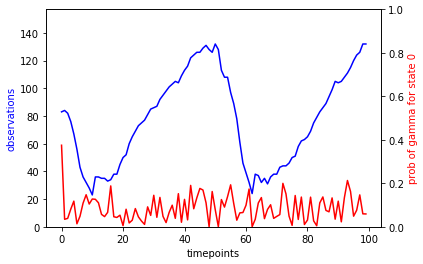
\includegraphics[width=\textwidth]{images/external-python-left}
    \caption{Observations an initial $\gamma$~probability for state~$0$ in the first iteration.}\label{fig:external-python-left}
  \end{subfigure}
  \begin{subfigure}[h]{0.48\textwidth}
    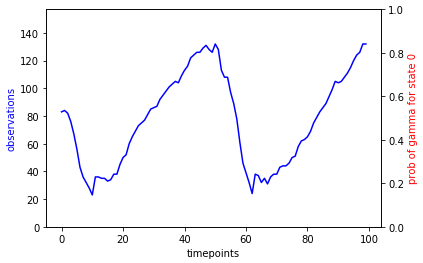
\includegraphics[width=\textwidth]{images/external-python-right}
    \caption{Observations and initial $\gamma$-probability for state~$0$ in the second iteration. The $\gamma$-values cannot be seen because they fail to be computed.}\label{fig:external-python-right}
  \end{subfigure}
  \caption[gamma-external]{Values of $\gamma$ obtained with this code.}\label{fig:gamma-external}
\end{figure}

\subsubsection{Algorithms}\label{sec:algorithms-python-external-underflow}

The term numerical underflow is used when the result of a calculation is smaller than the smallest minimum value that a computer can store in memory.
In Baum-Welch numerical underflow can occur in very large observations sequences because of the multiplication of probabilities.
A description of this problem and possible implementations to overcome it are described in this write-up: {\footnotesize\url{https://pdfs.semanticscholar.org/54dc/c2a758e7fa34b8c2ef19826f39f16c4d1731.pdf}}.

One solution involves using the $\log$ of probabilities to convert the multiplications into addition.
This process succeeds with the $\alpha$'s and $\beta$'s computed in the forwards-backwards algorithm, but not for the $\gamma$'s we compute as temporary variables, as they are already a sum of the $\alpha$'s.
Hence to avoid underflow, values of $\alpha$ and $\beta$ are normalized.
We compute
\begin{equation*}
  \hat{\alpha} = \frac{1}{\sum_{i=0}^N \alpha_i(t)}, \qquad \hat{\beta} = \frac{1}{\sum_{i=0}^{N-1}\beta_i(t)}
\end{equation*}
where $\hat{\alpha}$ and $\hat{\beta}$ denote the normalized values.
The $\gamma$ values are calculated as before, since the normalizers are cancelled.
But the $\xi$ values now have a slightly different formula.
\begin{align*}
  \gamma_i(t) &= \frac{\hat{\alpha}_i(t) \hat{\beta}_i(t)}{\sum_{j=1}^N \hat{\alpha}_j(t) \hat{\beta}_j(t)},
  \xi_{i, j}(t) &= \frac{\hat{\alpha}_i(t) a_{i, j} b_{j, t+1} \eta_{t+1} \hat{\beta}_{j}(t+1)}{\sum_{j=1}^N \hat{\alpha}_j(t) \hat{\beta}_j(t)} = \frac{\gamma_i(t) a_{i, j} b_{j, t+1} \eta_{t+1} \hat{\beta}_j(t+1)}{\hat{\beta}_i(t)}.
\end{align*}
% TODO figure out $\eta$ notation

We use this algorithm we same way we have the previous implementations: randomly initialize the parameters, train on the first run to obtain new parameter values, and continue using the algorithm to update hte parameters for all $\num{10000}$~runs.

\paragraph{Results}

Unfortunately the normalization steps again reduce the efficiency of this Python code, and it again takes an unreasonably long time to complete the iterations.
Again we try various modifications to the parameters, such as reducing their sizes and subsampling time steps, but we still cannot reach a reasonable level of efficiency with our code.

In order to prevent the program from running too long, we tried another solution in which we manually initialize the transition and emission matrices.
Since the robot appears to follow a roughly circular orbit, we induce our own ``radial states'' through the transition and emission matrices.
The general geometric schema of the states is shown in \cref{fig:radial-states}.
\begin{figure}[h]
  \centering
  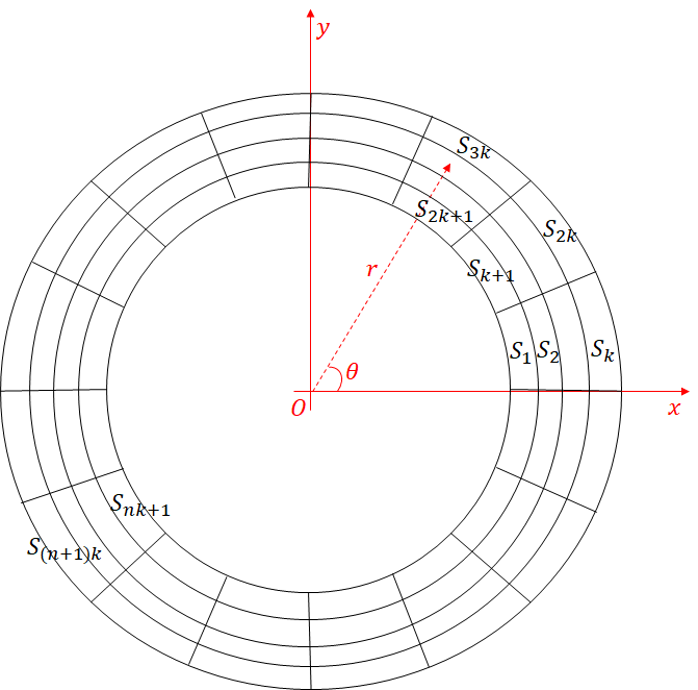
\includegraphics[width=0.5\textwidth]{images/AK7}
  \caption{Radial States}\label{fig:radial-states}
\end{figure}
The $\theta'$ range is also discretized, and the emission matrix~$E$ is initialized as follows.
If $x_i$ corresponds to the observation $\theta' \in [\theta_1', \theta_2']$, $S_T$ is the state corresponding to ${\theta \in [\theta_1, \theta_2]}$ and ${r \in [r_1, r_2]}$, and $\delta$ is a fixed positive real (exact value doesn't matter, since we normalize the matrix) then we set ${\Pr(X_t = s_i \mid S_T) = \delta}$ if one of the following lies within ${[\theta_1, \theta_2]}$:
\begin{align*}
  &\max \bigg( \arctan \Big(\frac{r_1\sin(\theta_1) + 1.5}{r_1\cos(\theta_1) + 1.5} \Big), \arctan \Big( \frac{r_1 \sin(\theta_2) + 1.5}{r_1 \cos(\theta_2) + 1.5} \Big), \arctan \Big( \frac{r_2 \sin(\theta_1) + 1.5}{r_2 \cos(\theta_1) + 1.5} \Big), \arctan \Big( \frac{r_2 \sin(\theta_2) + 1.5}{r_2 \cos(\theta_2) + 1.5} \Big) \bigg),\\
  &\min \bigg( \arctan \Big(\frac{r_1\sin(\theta_1) + 1.5}{r_1\cos(\theta_1) + 1.5} \Big), \arctan \Big( \frac{r_1 \sin(\theta_2) + 1.5}{r_1 \cos(\theta_2) + 1.5} \Big), \arctan \Big( \frac{r_2 \sin(\theta_1) + 1.5}{r_2 \cos(\theta_1) + 1.5} \Big), \arctan \Big( \frac{r_2 \sin(\theta_2) + 1.5}{r_2 \cos(\theta_2) + 1.5} \Big) \bigg).
\end{align*}
Otherwise set ${\Pr(X_t = s_i \mid S_T) = 0}$.
Finally normalize the matrix.

The transition matrix is initialized as follows.
If a state~$S$ corresponds to $\theta$~and~$r$, the probability of a transition to a state corresponding to any~$r$ and to the same, previous, or next~$\theta$ in the discretization is equal to $\delta$, and $0$ for all the other states.
Then normalize the matrix.

\paragraph{Results}

Here the Baum-Welch algorithm is able to converge for a small number of states ($3$~values of$r$ and $4$~values of $\theta$, for a total of $12$~states).
But with a larger number of states, the convergence of the computation is again too long in Python.

\subsection{Baum-Welch in Matlab}\label{sec:baum-welch-matlab}

With unsuccessful results form Python libraries, we next use the \texttt{\small hmmtrain} function of Matlab.
This function uses the observation sequence, transition matrix, and emission matrix to learn about the HMM and to predict the new transition and emission matrices.
This implementation is considerably faster than the Python implementations we used.
The transition and emission matrices converges about processing the first $\num{200}$ runs and took only about $\num{3}$~hours to run.

\subsubsection{Implementation and Choice of Parameters}\label{sec:choice-parameters}


One way to initialize the parameters $A$,~$B$, and $\pi$ of the Baum Welch algorithm is to do so randomly.
However, doing so means the algorithm takes a long time to converge.
By choosing initialization parameters close to what we expect the algorithm's output to be, we can decrease the number of steps that the algorithm requires to converge.

To initialize the transition matrix, we take advantage of the fact that the robot is moving rather slowly around the circle.
That is, in only one step, the robot is likely either to stay in the same state or move to a state with a location close to its previous state's location.
It will not make large transitions, e.g. from the bottom to the top of the circle, in a single step.
Thus it makes sense to initialize many values of the transition matrix to be~$0$, as there are only a small number of states to which the robot may transition from any given state.

Further, the Baum Welch converges to a local maximum.
And by changing the initial parameters we can change the local maximum to which the algorithm converges.
Thus we choose to initialize our transition matrix so that the states correspond to sections of the robot's path.
In \cref{fig:init-trans-pos} we show how we pick locations to guide our construction of the transition matrix.
\begin{figure}[h]
  \centering
  \begin{subfigure}[h]{0.48\textwidth}
    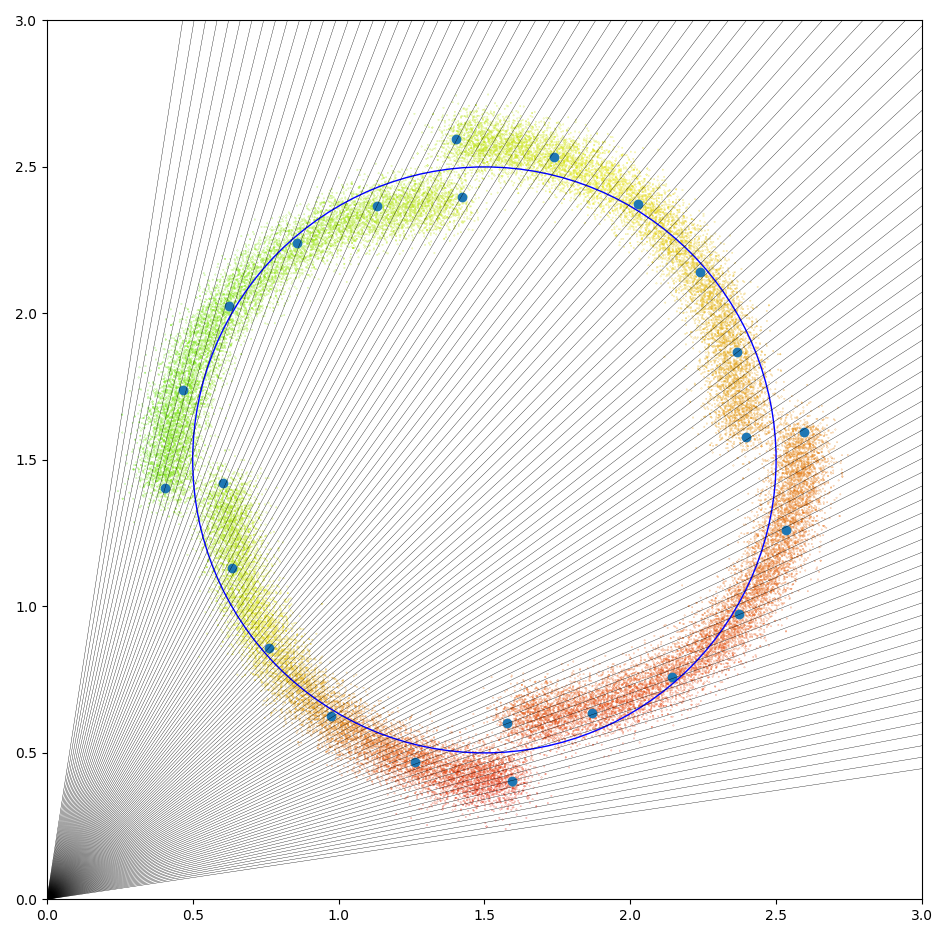
\includegraphics[width=\textwidth]{images/init-states-24}
    \caption{N = 24.}\label{fig:24-states}
  \end{subfigure}
  \begin{subfigure}[h]{0.48\textwidth}
    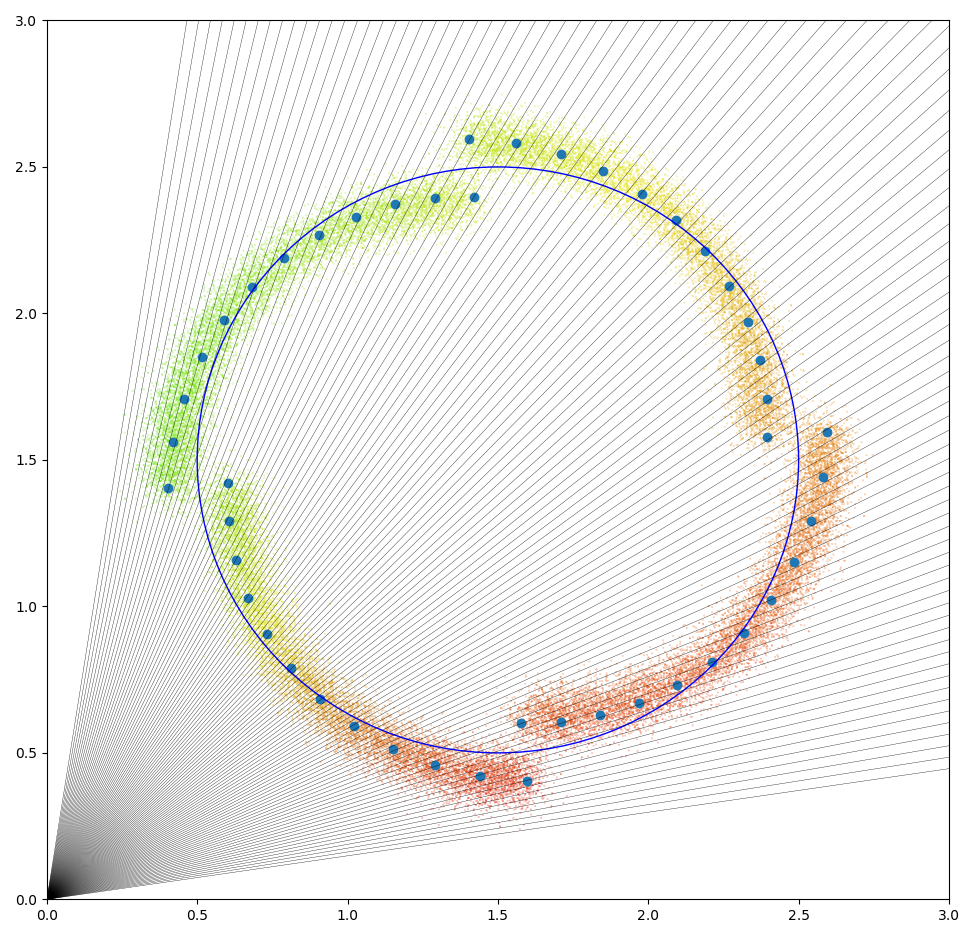
\includegraphics[width=\textwidth]{images/init-states-48}
    \caption{N = 48.}\label{fig:48-states}
  \end{subfigure}
  \caption{Initial state positions for different numbers of states.}\label{fig:init-trans-pos}
\end{figure}
We pick points along the robot's path and choose transition probabilities either that the robot stays in the same state or moves to the next state.
For example, for $4$~states, our initial transition matrix is
\begin{equation*}
  \begin{bmatrix}
    0.75 & 0.25 & 0    & 0\\
    0    & 0.75 & 0.25 & 0\\
    0    & 0    & 0.75 & 0.25\\
    0.25 & 0    & 0    & 0.75
  \end{bmatrix}
\end{equation*}

Further, we decide not to use any of the first $\num{200}$~time steps in our model.
The robot starts at~${(1.5, 1.5)}$, but by the time we start receiving labels at time~$\num{201}$, the robot has already reached its general orbit around its path.
We don't have any labels for the first~$\num{200}$ time steps, so using these values ends up making it more difficult for our algorithms to estimate the behavior of the robot at the tail of its runs, which is the behavior in which we are most interested to predict the $\num{1001}$st location.
When we try using these initial observations, our Baum Welch algorithm outputs a state to keep track of the values in the middle.
\Cref{fig:state-in-the-middle} shows how these initial observations result in points being assigned to a state that does not correspond to a useful location in the tail of the robot's path, but instead results in just a few points being assigned to this state instead of to a more reasonable location around the ring of the circle.
\begin{wrapfigure}{o}{0.5\textwidth}
  \centering
  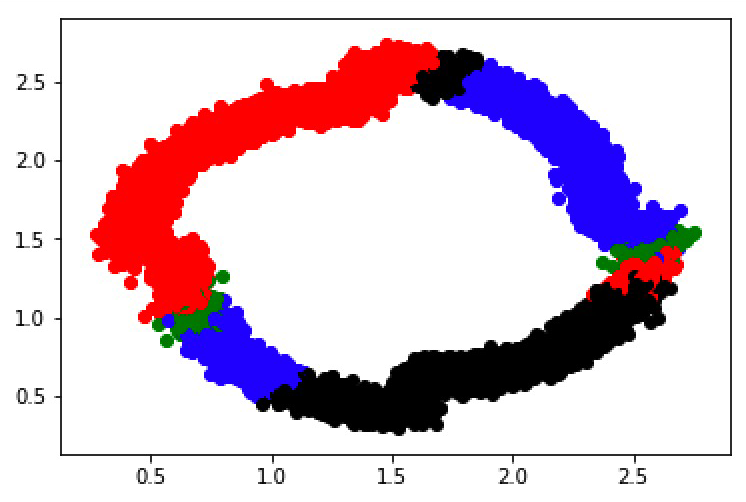
\includegraphics[width=0.48\textwidth]{images/state-in-the-middle}
  \caption[middle]{The green points are assigned to a state representing the middle of the circle through which the robot finishes moving by time~$200$.}\label{fig:state-in-the-middle}
\end{wrapfigure}

We also attempt to initialize the emission matrix.
After placing the initial state centers along the arcs of the robot's path, we assign each labeled point to the closest state based on the Euclidean distance between the point and the state's center.
Since we discretize the angles, we now determine the number of labeled points in each observation angle out of the total number of points assigned to the state.
This process gives us the initial values of our emission matrix.
Again, many of the values of this matrix are $0$, since a state that corresponds to the bottom right of the circle will never emit observations that correspond to angles close to~$\frac{\pi}{2}$.

However, this initialization of the emission matrix does not produce good results.
The large number of $0$'s present in the matrix tend to result in numerical errors when running the Matlab implementation.
We attempt to overcome this issue by adding an extremely small value, such as $0.00000001$, to the entries of the matrix, but we were unable to remove completely the numerical issues.
Randomly initializing the emission matrix does not create these numerical issues, so in our final implementation we use the randomly initialized matrix.

\paragraph{Results}

This implementation produces the best result, and we are able to achieve distinct states in a reasonable amount of computation time.
In the final mode, the Baum-Welch Matlab code is used to compute the transition and emission matrices before using the Viterbi algorithm to determine the most likely states.

\subsection{Viterbi}\label{sec:viterbi}

Viterbi is a dynamic programming algorithm that is used to predict the most likely hidden states.
However, Viterbi training can also be used for the training of a HMM.
We consider Viterbi training as an alternative to Baum-Welch training, which are computationally slow.
We describe both uses of Viterbi in this section.

\subsubsection{Algorithm}\label{sec:algorithm-viterbi}

The algorithm is used for predicting the hidden states for a path ${X = (x_1, x_2, \ldots, x_T)}$.
The hidden states are denoted as ${x_n \in S = \{S_1, s_2, \ldots, s_K\}}$, and the observations are denoted by ${Y = (y_1, y_2, \ldots, y_T) \in {\{1, 2, \ldots, N\}}^T}$.
Again, we use $N$ for the number of states, $K$ for the number of observations, $T$ for the number of time steps, and $A$ and $B$ with elements $a_{i, j}$ and $b_{i, k}$ for the transition and emission matrices, respectively.

The algorithm uses two tables of size~${K \times T}$.
\begin{itemize}
\item In the first table, each element~$T_1[i, j]$ of~$T_1$ stores the probability of the most likely path so far, which we denote by ${\hat{X} = (\hat{x}_1,\ldots,\hat{x}_j)}$.
  Here ${\hat{x}_j = s_j}$, which generates ${Y = (y_1, \ldots, y_j)}$.
\end{itemize}

The entries in the tables $T_1$~and~$T_2$ are filled in by
\begin{align*}
  T_i[i, j] &:= \max_k \{T_1[k, j-1]a_{k, i} b_{i, y_1}\},\\
  T_2[i, j] &:= \argmax_k \{T_1[k, j-1] a_{k, i} b_{i, y_1}\}.
\end{align*}
% TODO get notation correct

\subsubsection{Implementation of Viterbi for Predicting States}\label{sec:impl-viterbi-pred}

Because Viterbi is used for predicting states, it is the obvious next step after predicting the transition and emission matrices.
Hence after predicting the probabilities with Baum-Welch, we use this algorithm to predict the states.
We use Matlab's \texttt{\small{}hmmviterbi} function.
This algorithm performs efficiently for us and has no major problems in computing the hidden states.
The steps for using this algorithm are as follows:
\begin{enumerate}
\item Obtain the transition and emission matrices from the Baum-Welch algroithm.
\item Provide the transition matrix, emission matrix, and observations from the first run to the Viterbi algorithm.
  In this case we use $\num{1570}$~observations.
\item The Viterbi algorithm outputs an array containing the hidden states that correspond to the observations.
\item Repeat for all $\num{10000}$~runs.
\item At the end obtain a matrix of size ${\num{10000} \time 800}$.
\end{enumerate}
Note here that we use only $800$ observations (from $200$ to $\num{1000}$) for every run since these points lie withing the orbit and not in the middle of the circle.

\paragraph{Results}

We use three different numbers of states: $16$,~$24$, and~$48$.
After obtaining the states, the labels for the first $100$~runs are plotted to study if the Viterbi algorithm is successful in determining the states.
These results are displayed in \cref{fig:viterbi-states}.
The most visually clear assignment of states occurs with $24$~states, so we decide to use $24$~states in our final model.
\begin{figure}[h]
  \centering
  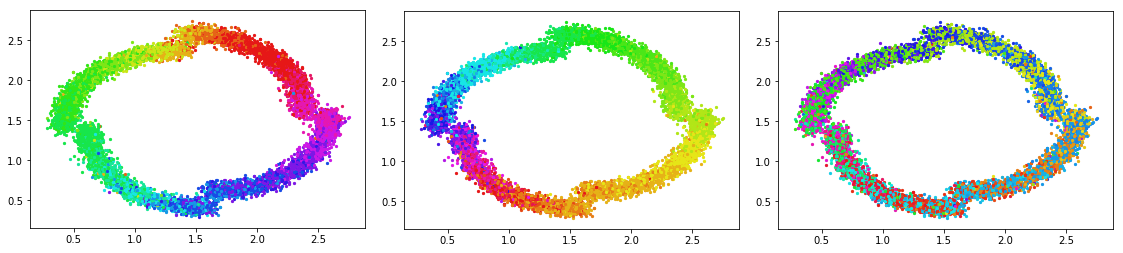
\includegraphics[width=0.9\textwidth]{images/viterbi-states}
  \caption{States formed by the Viterbi algorithm for $16$,~$24$, and~$48$ states.}\label{fig:viterbi-states}
\end{figure}

\subsection{Implementation of Viterbi Training}\label{sec:impl-viterbi-train}

Viterbi training, also knows as segmental $K$-means, works on the same principle as $K$-means.
The Viterbi algorithm is first used to predict the states of hte observations using randomly initialized transition and emission matrices.
After deriving the hidden states, the transition and emission matrices are then derived using the hidden states and observations.
These two steps are repeated until the matrices converge.
Unlike Buam-Welch, Viterbi training doesn't give the full conditional likelihood by only the maximum conditional likelihood, and hence is $1$~to~$2$ orders faster than Baum-Welch.

We implemented this algorithm from scratch in Python.
The steps of our implementation are as follows:
\begin{enumerate}
\item Randomly initialized the transition and emission matrices.
\item Use the transition matrix, emission matrix, and run~$1$ observations as the input.
\item Derive the hidden states, then derive the new transition and emission matrices using the hidden state sequence.
\item Repeat until convergence.
\item Use the new matrices to run Viterbi training on the observations from run~$2$.
\item Repeat for all $\num{10000}$~runs.
\end{enumerate}

\begin{figure}[h]
  \centering
  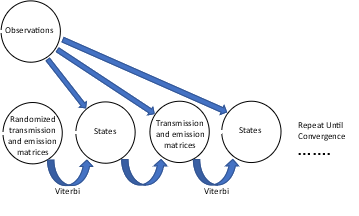
\includegraphics[width=0.7\textwidth]{images/viterbi-training}
  \caption{Viterbi Training}\label{fig:viterbi-training}
\end{figure}

\Cref{fig:viterbi-training} gives a pictorial representation of the Viterbi training algorithm and show that the same observation is used for predicting the hidden states and the emission and transition matrices again and again.
This process is repeated until convergence.

\paragraph{Results}

While optimistic that this algorithm would prove more efficient at training our HMM parameters than Baum-Welch, the results we obtained are not satisfactory.
We attempted this method several times, making a variety of small alterations, but never received a promising result when using it with the robot challenge.
The state sequence derived from this algorithm is not in any pattern.
Because the bot moves a limited distance every time step, there is no possibility of drastic changes in state between the two consecutive time steps.
Unfortunately, this algorithm produced large changes in state that did not follow any pattern.
We were unable to find a suitable solution to this algorithm after many trials, and thus decided to continue with using the Matlab HMM tools for our model.

\section{Finding the Location}\label{sec:finding-the-locat}

\begin{wrapfigure}{i}{0.3\textwidth}
  \begin{center}
    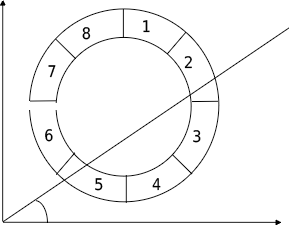
\includegraphics[width=0.28\textwidth]{images/two-intersection}
    \caption[multi-intersect]{Multiple Intersections Determined by One Angle}\label{fig:multi-intersect}
  \end{center}
\end{wrapfigure}
After finding the right state, transition matrix, and emission matrix, the next step is to find the locations corresponding to the states.
The project requires finding the location at the $\num{1001}$th~point.
However, because the bot does not move a large distance in every time step, we began by submitting simply the location of the $\num{1000}$th~step to check the accuracy of our methods.
Our first submission come from finding the $\num{1000}$th~location of runs $\num{6001}$~to~$\num{10000}$.
After verifying our methods here, we then proceed to predict the location of the $\num{1001}$st~point.

\subsection{Finding the $\num{1000}$th Point Using Median and Projections}\label{sec:find-num1000th-point}

The biggest concern in finding the location corresponding to tan angle is that there are multiple sections of the circle that fall on the same angle.
As seen in \cref{fig:multi-intersect}, the line determined by angle~$\theta$ passes through two regions of the circle.

\subsubsection{Using Labels to Map States to Locations}\label{sec:using-labels-map}

We use the labels for the first $\num{6000}$~runs to map the states produced from our algorithm to locations.
We then use these state locations to determine the location of the $\num{1000}$th~point in the final $\num{4000}$~runs.
\begin{enumerate}
\item Find the state of the $\num{1000}$th~point for runs $\num{6001}$~to~$\num{10000}$ using the Viterbi algorithm.
\item For each such point, find all labeled points that have the same state and discretized angle as this $\num{1000}$th point.
  This process solves the problem of every angle passing through multiple sections of the circle.
  Because the location of many points in the same state are given in the labels, it must be that region of the circle that is close to these datapoints.
\item If one or more labeled points are found with the same state and discretized angle, then the median of these points is determined and used as the location of the $\num{1000}$th~point.
\item If no points are found at the same angle and state, the take the median of all the labeled points in the same state (not just same state and same angle) and project this median on the line determined by the observation angle.
  Use this projection as the location of the $\num{1000}$th~point.
\item Repeat for runs $\num{6001}$~to~$\num{10000}$.
\end{enumerate}

\paragraph{Results}

The results from this algorithm are promising.
By predicting the $\num{1000}$th~point with the preceding algorithm, we obtain a Kaggle score of approximately~$0.28$.
Next we proceed to use this $\num{1000}$th~point to predict the location of the $\num{1001}$st~point.

\subsection{Finding the $\num{1001}$st Point Using Transition and Emission Matrices}\label{sec:find-num1001st-point}

In order to predict the position of the bot at the $\num{1001}$th time-step, it is essential to know the State and the value of the observed variable at time-step $\num{1001}$.
The approach we take for deriving this value is to utilize the Emission and Transition probability tables generated by the EM training and the mapping of bot-position to States generated by the Viterbi method.
The State at timestep $\num{1000}$ is known from the outcome of the Viterbi algorithm.
We scan the row in Transition probability matrix corresponding this State to locate the most likely''' ``next state''.
This is the State for which the Transition probability from $S_{\num{1000}}$ is maximum.
Once the value of $S_{\num{1001}}$ is identified, the Emission probability matrix is looked up to identify the most likely value of the variable corresponding to that state.
The process of doing this is similar: scan the row in the Emission probability matrix corresponding to $S_{\num{1001}}$, to locate the observation value that has highest emission probability.

\subsection{Finding the $\num{1001}$st Point Using Results From \Cref{sec:visu-cons-labels}.}\label{sec:finding-1001-angles}

In \cref{sec:visu-cons-labels} we plotted the distribution of~${\dif \theta}$ for all of the consecutive labels in the same run.
From the curve of \cref{fig:hist-dtheta} we make the assumption that the $\theta_{t+1}$ of step ${t+1}$ is chosen form a normal distribution of mean ${\theta_t + 0.125}$ and variance $0.125$.
The same way, the most probable value of $r_{t+1}$ knowing $r_t$ is $r_t + 0.0231$.

Therefore, another way to guess the $\num{1001}$st point knowing the $\num{1000}$th point is using the following formulas
\begin{align*}
  x_{\num{1001}} &= \Big( \sqrt{x_{\num{1000}}^2 + y_{\num{1000}}^2} + 0.0231 \Big) \cos \Big( \arctan \Big(\frac{y_{\num{1000}}}{x_{\num{1000}}} + 0.125 \Big) \Big),\\
  y_{\num{1001}} &= \Big( \sqrt{x_{\num{1000}}^2 + y_{\num{1000}}^2} + 0.0231 \Big) \sin \Big( \arctan \Big(\frac{y_{\num{1000}}}{x_{\num{1000}}} + 0.125 \Big) \Big).
\end{align*}
Note, depending on the signs of $x_{\num{1000}}$~and~$y_{\num{1000}}$, $\arctan \Big( \frac{y_{\num{1000}}}{x_{\num{1000}}} \Big)$ may need to be incremented by~$\pi$.
\Cref{fig:shifted-angles} shows our best guesses of the $\num{1000}$th positions for the final $\num{4000}$~runs in blue and our computed guess of the $\num{1001}$st position in red.
Implementing this strategy decreased our score error by~$0.01$ over the strategy of \cref{sec:find-num1001st-point}.
\begin{figure}[h]
  \centering
  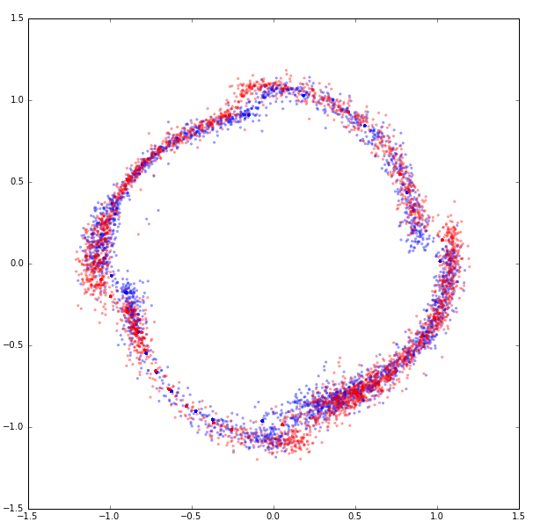
\includegraphics[width=0.6\textwidth]{images/AK8}
  \caption{Predicted locations.}\label{fig:shifted-angles}
\end{figure}

\section{Final Model}\label{sec:final-model}

For our final model we use the Matlab function \texttt{\small{}hmmtrain} as our implementation of Baum-Welch, as described in \cref{sec:baum-welch-matlab}.
We use the manually constructed transition matrix and randomly initialized emission matrix as described in \cref{sec:choice-parameters}, using $24$~states and $1570$~discrete angles.
We use the final $800$~timesteps of each run, avoid the first $200$~steps during which the robot may not have reached its tail behavior.
Then we use Matlab's \texttt{\small{}hmmviterbi} function, as explained in \cref{sec:viterbi}, to determine the most likely states given the observation angles and matrices output from \texttt{\small{}hmmtrain}.
Finally we use the method of \cref{sec:finding-1001-angles} to determine the location of the $\num{1001}$st point.
Our final model achieves an accuracy score of~$\bm{0.26233}$.

% TODO how to use BW if it runs better

\section{Conclusions}\label{sec:conclusions}

\end{document}

